% !TEX program = xelatex
\documentclass[aspectratio=169, 11pt]{ctexbeamer}

% ====== 主题 ======
\usetheme{metropolis}
\metroset{
    progressbar=frametitle,
    numbering=fraction,
    block=fill,
}

% ====== 宏包 ======
\usepackage{graphicx}
\usepackage{booktabs}
\usepackage{amsmath, amssymb}
\usepackage{tikz}
\usepackage{appendixnumberbeamer}
\usepackage{multicol}
\usepackage{array}           % >{\bfseries}r column spec
\usepackage[normalem]{ulem}  % \sout{} for strikethrough

\usetikzlibrary{arrows.meta, positioning, shapes.geometric, calc}

% ====== 颜色 ======
\definecolor{mDarkTeal}{HTML}{23373B}
\definecolor{mLightBrown}{HTML}{EB811B}
\definecolor{mLightGreen}{HTML}{14B03D}
\definecolor{mAlertRed}{HTML}{CC0000}
\definecolor{mSoftBlue}{HTML}{3366CC}

\setbeamercolor{alerted text}{fg=mLightBrown}

% ====== 图路径 ======
\graphicspath{{../results/figures/baseline/}{../reports/uq_validation/}}

% ====== 标题 ======
\title{UQ-ORION}
\subtitle{面向恶劣天气的不确定性感知端到端自动驾驶安全扩展}
\date{2026 年 4 月 1 日}
\author{}
\institute{}

\begin{document}

% ============================================================
\maketitle

% ============================================================
\begin{frame}{目录}
    \setbeamertemplate{section in toc}[sections numbered]
    \tableofcontents[hideallsubsections]
\end{frame}

% ============================================================
\section{背景与动机}

% ============================================================
\begin{frame}{ORION：VLM-based 端到端自动驾驶}

\begin{columns}[T]
\begin{column}{0.55\textwidth}
\textbf{ORION}（ICCV 2025）流程：
\begin{enumerate}
    \item 多视角图像 $\to$ EVAViT encoder
    \item QT-Former 场景理解
    \item Qwen VLM 推理 + 规划
    \item VAE 解码 $\to$ 轨迹
\end{enumerate}

\vspace{0.5em}
\textbf{优势}：利用 VLM 的世界知识做驾驶决策

\vspace{0.5em}
\textbf{问题}：在恶劣天气下\alert{过度自信}
\begin{itemize}
    \item 不知道``自己看不清了''
    \item 依然做出激进决策
\end{itemize}
\end{column}

\begin{column}{0.4\textwidth}
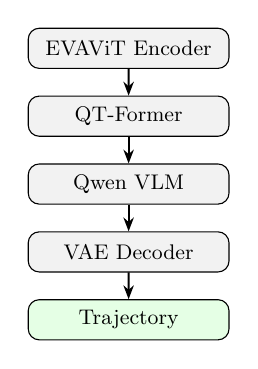
\begin{tikzpicture}[
    box/.style={draw, rounded corners, minimum width=3cm, minimum height=0.6cm, font=\small, fill=gray!10},
    arr/.style={-{Stealth[length=5pt]}, thick},
    scale=0.85, transform shape
]
    \node[box] (enc) {EVAViT Encoder};
    \node[box, below=0.4cm of enc] (qt) {QT-Former};
    \node[box, below=0.4cm of qt] (vlm) {Qwen VLM};
    \node[box, below=0.4cm of vlm] (vae) {VAE Decoder};
    \node[box, below=0.4cm of vae, fill=green!10] (traj) {Trajectory};

    \draw[arr] (enc) -- (qt);
    \draw[arr] (qt) -- (vlm);
    \draw[arr] (vlm) -- (vae);
    \draw[arr] (vae) -- (traj);
\end{tikzpicture}
\end{column}
\end{columns}
\end{frame}

% ============================================================
\begin{frame}{核心发现：恶劣天气碰撞率放大 161$\times$}

\begin{table}
\centering
\begin{tabular}{lcc>{\bfseries}r}
\toprule
\textbf{指标} & \textbf{Normal} & \textbf{Adverse} & \textbf{倍数} \\
\midrule
L2@3s & 2.38m & 1.78m & $0.75\times$ \\
Col@1s & 0.02\% & 1.78\% & $89\times$ \\
Col@3s & 0.01\% & 1.61\% & $161\times$ \\
\bottomrule
\end{tabular}
\end{table}

\vspace{0.5em}

\begin{alertblock}{反直觉发现}
\begin{itemize}
    \item 恶劣天气的 L2 误差反而\textbf{更低}（低速→短轨迹→天然低 L2）
    \item 但碰撞率高出 \textbf{161 倍}
    \item \textbf{L2 轨迹精度 $\neq$ 安全性}，开环指标看不出问题
\end{itemize}
\end{alertblock}

\vspace{0.3em}
{\small \textcolor{gray}{数据来源：Bench2Drive 验证集，12,806 个样本（开环评估）}}\\
{\scriptsize \textcolor{gray}{\textbf{Adverse 判定}：Weather ID $\notin \{0,1,2,3\}$，即非 ClearNoon/ClearSunset/CloudyNoon/CloudySunset 的所有条件（含晴天夜间 ClearNight）均归为 Adverse（共 19 种，10,097 帧）。}}
\end{frame}

% ============================================================
% ----------------------------------------------------------
\begin{frame}[t]{阶段性研究问题}

\small
\textbf{本阶段不刷榜 L2}，在\textbf{冻结 ORION 主干}上回答四个问题：

\vspace{0.35em}
\begin{enumerate}\setlength{\itemsep}{0.45em}
    \item[\textbf{Q1}] \textbf{能否监测？}\\
    从冻结视觉 patch tokens 估计「当前感知有多差」（UQ score）
    \item[\textbf{Q2}] \textbf{能否改行为？}\\
    不修改主干权重，用 FiLM 条件调制规划（QT-Former + VAE）
    \item[\textbf{Q3}] \textbf{代价是什么？}\\
    碰撞率改善是否以 Normal 轨迹退化、效率下降为代价？
    \item[\textbf{Q4}] \textbf{能否空间化？}\\
    不确定性能否从全局标量扩展到 BEV 空间热力图？
\end{enumerate}

\vspace{0.35em}
\footnotesize
\textcolor{gray}{评估：开环 12,806 帧 + 50 场景回放式闭环；Adverse = Weather ID $\notin \{0,1,2,3\}$。}
\end{frame}

\section{总体框架}

% ============================================================
\begin{frame}{整体架构：轻量 UQ + 双层 FiLM 注入}

\begin{center}
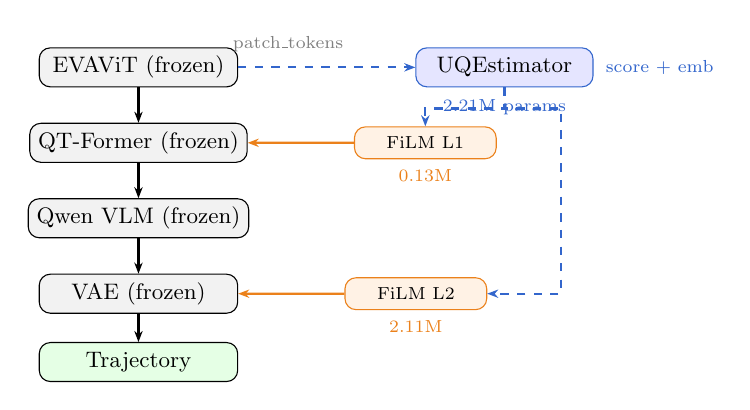
\begin{tikzpicture}[
    box/.style={draw, rounded corners, minimum width=2.8cm, minimum height=0.55cm, font=\small, fill=gray!10},
    uqbox/.style={draw, rounded corners, minimum width=2.5cm, minimum height=0.55cm, font=\small, fill=blue!10, draw=mSoftBlue},
    filmbox/.style={draw, rounded corners, minimum width=2cm, minimum height=0.45cm, font=\scriptsize, fill=orange!10, draw=mLightBrown},
    arr/.style={-{Stealth[length=4pt]}, thick},
    darr/.style={-{Stealth[length=4pt]}, thick, dashed, color=mSoftBlue},
    scale=0.9, transform shape
]
    \node[box] (enc) {EVAViT (frozen)};
    \node[box, below=0.5cm of enc] (qt) {QT-Former (frozen)};
    \node[box, below=0.5cm of qt] (vlm) {Qwen VLM (frozen)};
    \node[box, below=0.5cm of vlm] (vae) {VAE (frozen)};
    \node[box, below=0.4cm of vae, fill=green!10] (traj) {Trajectory};

    % UQ
    \node[uqbox, right=2.5cm of enc] (uq) {UQEstimator};
    \node[font=\scriptsize, below=0.05cm of uq, text=mSoftBlue] (uqp) {2.21M params};

    % FiLM
    \node[filmbox, right=1.5cm of qt] (film1) {FiLM L1};
    \node[font=\scriptsize, below=0.02cm of film1, text=mLightBrown] {0.13M};
    \node[filmbox, right=1.5cm of vae] (film2) {FiLM L2};
    \node[font=\scriptsize, below=0.02cm of film2, text=mLightBrown] {2.11M};

    % Arrows
    \draw[arr] (enc) -- (qt);
    \draw[arr] (qt) -- (vlm);
    \draw[arr] (vlm) -- (vae);
    \draw[arr] (vae) -- (traj);

    % UQ connections
    \draw[darr] (enc.east) -- ++(0.8,0) |- (uq.west);
    \draw[darr] (uq.south) -- ++(0,-0.3) -| (film1.north);
    \draw[darr] (uq.south) -- ++(0,-0.3) -- ++(0.8,0) |- (film2.east);

    % FiLM inject
    \draw[arr, color=mLightBrown] (film1.west) -- (qt.east);
    \draw[arr, color=mLightBrown] (film2.west) -- (vae.east);

    % Labels
    \node[font=\scriptsize, above right=0.1cm and -0.2cm of enc.east, text=gray] {patch\_tokens};
    \node[font=\scriptsize, right=0.05cm of uq.east, text=mSoftBlue] {score + emb};
\end{tikzpicture}
\end{center}

\vspace{0.3em}

\begin{columns}[T]
\begin{column}{0.48\textwidth}
\textbf{设计原则}：
\begin{itemize}
    \item 零主干微调
    \item 新增参数 4.45M（主干的 0.45\%）
    \item 一行开关切换
\end{itemize}
\end{column}
\begin{column}{0.48\textwidth}
\textbf{FiLM 调制}：$\text{out} = \gamma \odot \text{in} + \beta$
\begin{itemize}
    \item L1：调制场景理解
    \item L2：调制轨迹规划
    \item Identity 初始化保证无损
\end{itemize}
\end{column}
\end{columns}
\end{frame}

% ============================================================
\section{UQEstimator}

% ----------------------------------------------------------
\begin{frame}{UQEstimator：模块定位}

\begin{columns}[T]
\begin{column}{0.52\textwidth}
\textbf{做什么？}
\begin{itemize}
    \item 读取 ORION \textbf{frozen} EVAViT 的 patch tokens
    \item 输出 \textbf{uncertainty\_score} $\in (0,1)$（标量）
    \item 输出 \textbf{uncertainty\_embedding} $\in \mathbb{R}^{256}$（供 FiLM）
\end{itemize}

\vspace{0.4em}
\textbf{不做什么？}
\begin{itemize}
    \item 不微调 Vision / QT-Former / VLM / VAE
    \item 不直接预测轨迹 L2 或碰撞
    \item 与 BEV 不确定性模块独立（见 Phase\,2）
\end{itemize}

\vspace{0.4em}
\textbf{代码位置}：\texttt{uq\_estimator/}，训练 \texttt{scripts/train\_uq.py}
\end{column}

\begin{column}{0.44\textwidth}
\begin{table}
\centering
\small
\begin{tabular}{lr}
\toprule
\textbf{项} & \textbf{值} \\
\midrule
参数量 & \textbf{2.21M} \\
上限目标 & $<$ 5M \\
训练显存 & $<$ 5GB \\
训练时长 & $\sim$100\,min \\
Val Spearman & \textbf{0.97} \\
\bottomrule
\end{tabular}
\end{table}

\vspace{0.3em}
{\scriptsize 推理时通过 forward hook 捕获 score，\\不改动 ORION 主推理图。}
\end{column}
\end{columns}
\end{frame}

% ----------------------------------------------------------
\begin{frame}{UQEstimator：端到端数据流}

\begin{center}
\begin{tikzpicture}[
    block/.style={draw, rounded corners, minimum height=0.55cm, font=\scriptsize, align=center, inner sep=4pt},
    patch/.style={block, fill=blue!8, minimum width=2.65cm},
    stat/.style={block, fill=orange!10, minimum width=2.2cm},
    fuse/.style={block, fill=green!10, minimum width=2.55cm},
    uqout/.style={block, fill=mSoftBlue!15, minimum width=2.15cm, draw=mSoftBlue},
    arr/.style={-{Stealth[length=3pt]}, thick, color=black!65},
    node distance=0.52cm,
    scale=0.88, transform shape
]
    % Patch 分支（左）
    \node[patch] (in) {patch\_tokens\\$[B,6,1600,1024]$};
    \node[patch, below=of in] (proj) {Linear $1024\!\to\!256$};
    \node[patch, below=of proj] (dec) {2$\times$ TransformerDecoder\\16 queries $\times$ patches};
    \node[patch, below=of dec] (pv) {视角 mean $\to$ $[B,256]$};

    % Stat 分支（右）：底边与 pv 对齐；加大左右间距
    \node[stat, anchor=south] (stproj) at ($(pv.south)+(3.4cm,0)$)
        {Linear $5\!\to\!64$\\+ GELU + LN};
    \node[stat, above=of stproj] (stin) {stat\_features\\$[B,5]$};

    % 汇合点在两分支正下方；Fusion 再下移，留出清晰间距
    \coordinate (jmerge) at ($(pv.south)!0.5!(stproj.south)+(0,-0.65)$);
    \node[fuse] (cat) at ($(jmerge)+(0,-0.95)$)
        {concat $\to$ Fusion MLP\\$320\!\to\!512\!\to\!256$};
    \node[uqout, below left=0.55cm and 1.15cm of cat] (score) {score\_head\\Sigmoid $\to [B,1]$};
    \node[uqout, below right=0.55cm and 1.15cm of cat] (emb) {embed\_head\\LN $\to [B,256]$};

    % 主链
    \draw[arr] (in) -- (proj) -- (dec) -- (pv);
    \draw[arr] (stin) -- (stproj);

    % 汇入：先竖直离开节点，再水平汇到 jmerge，最后进入 Fusion
    \draw[arr] (pv.south) -- (pv.south |- jmerge);
    \draw[arr] (stproj.south) -- (stproj.south |- jmerge);
    \draw[arr] (pv.south |- jmerge) -- (jmerge);
    \draw[arr] (stproj.south |- jmerge) -- (jmerge);
    \draw[arr] (jmerge) -- (cat.north);

    % 分叉至双头：竖直下降 → 水平总线 → 分别进入两输出头
    \coordinate (jsplit) at ($(cat.south)+(0,-0.28)$);
    \coordinate (busL) at (jsplit -| score.north);
    \coordinate (busR) at (jsplit -| emb.north);
    \draw[arr] (cat.south) -- (jsplit);
    \draw[thick, color=black!65] (busL) -- (busR);
    \draw[arr] (busL) -- (score.north);
    \draw[arr] (busR) -- (emb.north);
\end{tikzpicture}
\end{center}

\vspace{0.2em}
\begin{center}
\scriptsize 训练只对 \textbf{score} 反传；embedding 在 ORION 推理中与 Score-Gated FiLM 结合。
\end{center}
\end{frame}

% ----------------------------------------------------------
\begin{frame}[t]{Patch 分支（1/2）：Cross-Attention 聚合}

\small
\textbf{为何需要 Decoder？}
\begin{itemize}\setlength{\itemsep}{0.25em}
    \item 单帧 $6 \times 1600$ patches，直接 mean pool 会丢失空间结构
    \item \textbf{16 个可学习 query} 对全图 patch 做 cross-attention
    \item 2 层 \texttt{TransformerDecoderLayer}（$d{=}256$，8 heads）
    \item 再对 6 视角的 query 输出做 mean $\to$ $[B,256]$
\end{itemize}

\vspace{0.6em}
\textbf{数据流（每视角）}
\begin{center}
\footnotesize
patch tokens $\xrightarrow{\text{Linear}}$ patch 序列
$\xrightarrow{\text{Decoder}}$ 16 queries
$\xrightarrow{\text{mean}}$ 256-d $\xrightarrow{\text{6-view mean}}$ $[B,256]$
\end{center}

\vspace{0.6em}
\textbf{消融}：\texttt{use\_transformer\_decoder=false}
\begin{itemize}\setlength{\itemsep}{0.2em}
    \item 退化为 patch 维 mean pool（更快、表达能力更弱）
\end{itemize}
\end{frame}

% ----------------------------------------------------------
\begin{frame}[t]{Patch 分支（2/2）：张量约定与训练}

\begin{columns}[T]
\begin{column}{0.52\textwidth}
\small
\textbf{输入张量约定}
\vspace{0.2em}

\begin{table}
\centering
\footnotesize
\renewcommand{\arraystretch}{1.15}
\begin{tabular}{@{}ll@{}}
\toprule
\textbf{符号} & \textbf{形状} \\
\midrule
patch\_tokens & $[B,6,1600,1024]$ \\
投影后 & $[B,6,1600,256]$ \\
queries & $[B,6,16,256]$ \\
视角聚合后 & $[B,256]$ \\
\bottomrule
\end{tabular}
\end{table}

\vspace{0.5em}
\footnotesize
\textcolor{gray}{EVAViT 输出 $D{=}1024$；UQEstimator 内先投影到 $d{=}256$ 再进 Decoder。}
\end{column}

\begin{column}{0.44\textwidth}
\small
\textbf{训练与工程}
\begin{itemize}\setlength{\itemsep}{0.3em}
    \item \texttt{n\_patches\_subsample=256}：每视角随机子采样 patch，加速训练
    \item Stage 0 特征缓存：12,806 帧 $\to$ \texttt{data/features/*.pt}
    \item 推理全量 1600 patch / 视角（与训练子采样可不同）
\end{itemize}

\vspace{0.4em}
\textbf{参数量}
\begin{itemize}\setlength{\itemsep}{0.2em}
    \item Patch 投影 + 2$\times$ Decoder 占 UQEstimator 主体
    \item 总模型约 \textbf{2.24M}（上限 5M）
\end{itemize}
\end{column}
\end{columns}
\end{frame}

% ----------------------------------------------------------
\begin{frame}[t]{统计特征分支（1/2）：5 维描述子}

\small
\textbf{来源}：\texttt{compute\_stat\_features(tokens)}（\texttt{dataset.py}）\\
从 Stage 0 缓存的 patch tokens 离线计算，\textbf{不增加 ORION 主推理计算图}。

\vspace{0.5em}
\begin{center}
\footnotesize
\renewcommand{\arraystretch}{1.2}
\begin{tabular}{@{}c l p{6.5cm}@{}}
\toprule
\textbf{\#} & \textbf{特征} & \textbf{设计直觉} \\
\midrule
0 & patch 激活方差均值 & 表征是否``发散''、不稳定 \\
1 & 跨 patch softmax 熵 & 归一化到 $[0,1]$；熵高 $\Rightarrow$ 注意力分散 \\
2 & 跨视角 token 余弦相似度 & 多相机表征是否一致 \\
3 & 激活绝对值均值 & 整体信号强度 \\
4 & 激活最大值均值 & 是否存在异常强响应 patch \\
\bottomrule
\end{tabular}
\end{center}

\vspace{0.5em}
\footnotesize
\textcolor{gray}{5 维原始特征 $\to$ 模型内 Linear$(5\!\to\!64)$ + GELU + LayerNorm，再与 Patch 分支 $[B,256]$ concat。}
\end{frame}

% ----------------------------------------------------------
\begin{frame}[t]{统计特征分支（2/2）：结构与消融}

\begin{columns}[T]
\begin{column}{0.48\textwidth}
\small
\textbf{分支结构}
\vspace{0.15em}

\begin{center}
\begin{tikzpicture}[
    block/.style={draw, rounded corners, font=\footnotesize, align=center,
        minimum width=2.1cm, minimum height=0.48cm, inner sep=2pt},
    arr/.style={-{Stealth[length=3pt]}, thick, color=black!65},
    node distance=0.4cm,
    scale=0.88, transform shape
]
    \node[block, fill=orange!12] (in) {stat\_features\\$[B,5]$};
    \node[block, fill=orange!12, below=of in] (proj) {Linear $5\!\to\!64$\\GELU + LN};
    \node[block, fill=green!10, below=of proj] (cat) {concat\\$[B,320]$};
    \node[block, fill=blue!8, left=1.5cm of cat] (pv) {Patch 分支\\$[B,256]$};
    \draw[arr] (in) -- (proj);
    \draw[arr] (proj) -- (cat);
    \draw[arr] (pv.east) -- (cat.west);
\end{tikzpicture}
\end{center}

\vspace{0.2em}
\footnotesize
与 Patch 分支在 Fusion MLP 前拼接：$256 + 64 = 320$。
\end{column}

\begin{column}{0.48\textwidth}
\small
\textbf{工程与消融}
\begin{itemize}\setlength{\itemsep}{0.28em}
    \item \textbf{消融}：\texttt{use\_stat\_features=false} 时整路跳过，Fusion 输入仅 $[B,256]$
    \item \textbf{缓存}：可选 \texttt{stat\_cache.pt}，避免每个 epoch 重算 5 维特征
    \item \textbf{互补}：Patch 路做空间聚合；统计路无 attention、可解释，显式编码分布形态
\end{itemize}
\end{column}
\end{columns}

\vfill
\hrule height 0.4pt
\vspace{0.35em}
\footnotesize
\textbf{设计取舍：}
去掉统计分支（\texttt{no\_stat}）时劣天气分离度与 Spearman 通常下降；
保留成本极低（$5\!\to\!64$ 投影 + 固定公式，不增加 ORION 推理开销）。
\end{frame}

% ----------------------------------------------------------
\begin{frame}[t]{损失函数（1/4）：监督对象与总目标}

\small
\textbf{训练监督谁？}
\begin{itemize}\setlength{\itemsep}{0.25em}
    \item 仅对 \textbf{score\_head} 输出 $\hat{s}\in[0,1]$（Sigmoid）计算损失；\texttt{embed\_head} 无直接监督
    \item 标签 $t$ 为 Stage 1a 伪标签（patch 统计 + weather 校准），形状 $[B,1]$
    \item 实现：\texttt{uq\_estimator/losses.py} $\to$ \texttt{CombinedUQLoss}
\end{itemize}

\vspace{0.5em}
\textbf{总损失（默认权重）}
\[
\mathcal{L}_{\text{total}}
= \underbrace{\mathrm{MSE}(\hat{s}, t)}_{\mathcal{L}_{\text{reg}}}
+ \underbrace{\lambda_{\text{cal}}\cdot\frac{1}{\mathrm{std}(\hat{s})+\epsilon}}_{\mathcal{L}_{\text{cal}},\;\lambda_{\text{cal}}=0.1}
+ \underbrace{\lambda_{\text{rank}}\cdot\mathcal{L}_{\text{rank}}}_{\lambda_{\text{rank}}=0.5}
\]

\vspace{0.4em}
\footnotesize
\texttt{forward} 返回字典：\texttt{total}, \texttt{regression}, \texttt{ranking}, \texttt{calibration}（便于 TensorBoard / 日志分项监控）。
\end{frame}

% ----------------------------------------------------------
\begin{frame}[t]{损失函数（2/4）：回归项 $\mathcal{L}_{\text{reg}}$}

\begin{columns}[T]
\begin{column}{0.52\textwidth}
\small
\textbf{定义}
\[
\mathcal{L}_{\text{reg}} = \frac{1}{B}\sum_{i=1}^{B}(\hat{s}_i - t_i)^2
\]

\textbf{作用}
\begin{itemize}\setlength{\itemsep}{0.28em}
    \item 拟合伪标签\textbf{绝对数值}：劣天气帧应更接近 $t\approx 1$，正常帧更接近 $0$
    \item 提供主监督信号，决定 score 的标定尺度
\end{itemize}

\vspace{0.4em}
\textbf{局限（单独 MSE 不够）}
\begin{itemize}\setlength{\itemsep}{0.22em}
    \item 对 batch 内\textbf{相对排序}约束弱：多个样本可共同塌缩到 batch 均值附近仍得较低 MSE
    \item 故需排序项 + 校准项配合（见后两页）
\end{itemize}
\end{column}

\begin{column}{0.44\textwidth}
\small
\textbf{伪标签 $t$ 从何而来？}
\begin{itemize}\setlength{\itemsep}{0.25em}
    \item \texttt{generate\_labels.py}：由 patch token 统计量组合
    \item v3：叠加 weather ID 校准，与开环 Adverse 划分对齐
    \item $t\in[0,1]$，连续值而非二分类 0/1
\end{itemize}

\vspace{0.5em}
\begin{block}{与 embed 的关系}
\footnotesize
回归只塑造 \textbf{score}；embedding 通过共享 Fusion 层间接受影响，但无独立 MSE/对比损失。
\end{block}
\end{column}
\end{columns}
\end{frame}

% ----------------------------------------------------------
\begin{frame}[t]{损失函数（3/4）：校准项 $\mathcal{L}_{\text{cal}}$（防塌缩）}

\small
\textbf{定义}（对当前 mini-batch 内预测分数求标准差）
\[
\mathcal{L}_{\text{cal}} = \lambda_{\text{cal}}\cdot\frac{1}{\mathrm{std}(\hat{s})+\epsilon},
\quad \lambda_{\text{cal}}=0.1,\;\epsilon=10^{-6}
\]

\vspace{0.35em}
\textbf{直觉}
\begin{itemize}\setlength{\itemsep}{0.25em}
    \item $\mathrm{std}(\hat{s})\downarrow$ $\Rightarrow$ $\mathcal{L}_{\text{cal}}\uparrow$：惩罚``整批预测几乎相同''
    \item 防止模型退化为常数输出（例如全预测 $\approx 0.5$），保留 batch 内可分辨度
    \item 与 $\mathcal{L}_{\text{reg}}$ 互补：MSE 管``对准标签''，校准管``别把方差压没''
\end{itemize}

\vspace{0.35em}
\begin{columns}[T]
\begin{column}{0.48\textwidth}
\footnotesize
\textbf{实现细节}
\begin{itemize}\setlength{\itemsep}{0.2em}
    \item \texttt{pred\_score.std()}：PyTorch 默认无偏估计（$n{-}1$ 分母）
    \item \textbf{$B{=}1$ 时 std 为 NaN}：训练配置 \texttt{batch\_size=64}，勿长期用 $B{=}1$ 调试
\end{itemize}
\end{column}
\begin{column}{0.48\textwidth}
\footnotesize
\textbf{消融}
\begin{itemize}\setlength{\itemsep}{0.2em}
    \item \texttt{configs/uq\_ablation\_no\_cal.yaml}：\texttt{use\_calibration: false} $\Rightarrow$ $\lambda_{\text{cal}}{=}0$
    \item 关闭后 score 分布可能变窄，Normal/Adverse 分离度下降
\end{itemize}
\end{column}
\end{columns}
\end{frame}

% ----------------------------------------------------------
\begin{frame}[t]{损失函数（4/4）：排序项与组合}

\begin{columns}[T]
\begin{column}{0.54\textwidth}
\small
\textbf{成对排序 $\mathcal{L}_{\text{rank}}$}
\begin{itemize}\setlength{\itemsep}{0.22em}
    \item 枚举 batch 内所有满足 $t_i > t_j$ 的样本对 $(i,j)$
    \item 用 \texttt{nn.MarginRankingLoss(margin=0.1)}，约束
    \[
    \hat{s}_i \geq \hat{s}_j + 0.1
    \]
    \item 若无有效对（如标签全相等）$\Rightarrow$ 返回 $0$（\texttt{requires\_grad=True}）
    \item 复杂度：每 batch 最多 $O(B^2)$ 对；$B{=}64$ 时约 $\leq 2016$ 对
\end{itemize}

\vspace{0.35em}
\footnotesize
\textbf{小例子}（$B{=}3$）：若 $t=[0.2,\,0.5,\,0.9]$，有效对为
$(2,0),(2,1),(1,0)$ 共 3 对；要求 $\hat{s}_2>\hat{s}_0$，$\hat{s}_2>\hat{s}_1$，$\hat{s}_1>\hat{s}_0$（均带 margin）。
\end{column}

\begin{column}{0.42\textwidth}
\small
\textbf{YAML 消融（\texttt{train\_uq.py} 置 $\lambda{=}0$）}
\footnotesize
\renewcommand{\arraystretch}{1.1}
\begin{tabular}{@{}ll@{}}
\toprule
\textbf{配置} & \textbf{关闭项} \\
\midrule
\texttt{no\_ranking} & $\mathcal{L}_{\text{rank}}$ \\
\texttt{no\_cal} & $\mathcal{L}_{\text{cal}}$ \\
\texttt{no\_stat} & 统计分支 \\
\texttt{no\_decoder} & Transformer Decoder \\
\bottomrule
\end{tabular}

\vspace{0.45em}
\textbf{三项分工}
\begin{itemize}\setlength{\itemsep}{0.18em}
    \item $\mathcal{L}_{\text{reg}}$：绝对值回归
    \item $\mathcal{L}_{\text{cal}}$：batch 内分散度
    \item $\mathcal{L}_{\text{rank}}$：相对序关系（劣天气 $>$ 正常）
\end{itemize}
\end{column}
\end{columns}
\end{frame}

% ----------------------------------------------------------
\begin{frame}[t]{score vs embedding（1/2）：Stage 1b 谁有监督？}

\small
\textbf{网络分叉}（\texttt{uq\_estimator/model.py}）
\vspace{0.2em}

\begin{center}
\begin{tikzpicture}[
    block/.style={draw, rounded corners, font=\footnotesize, align=center,
        minimum width=2.0cm, minimum height=0.48cm, inner sep=2pt},
    arr/.style={-{Stealth[length=3pt]}, thick, color=black!65},
    node distance=0.38cm,
    scale=0.92, transform shape
]
    \node[block, fill=green!10] (fus) {Fusion\\$[B,256]$};
    \node[block, fill=mSoftBlue!15, below left=0.5cm and 0.9cm of fus] (sc) {score\_head\\$\to [B,1]$};
    \node[block, fill=orange!12, below right=0.5cm and 0.9cm of fus] (em) {embed\_head\\$\to [B,256]$};
    \node[font=\footnotesize, below=0.12cm of sc, text=red!70!black] {有 $\mathcal{L}_{\text{UQ}}$};
    \node[font=\footnotesize, below=0.12cm of em, text=gray] {无直接 loss};
    \draw[arr] (fus.south west) -- (sc.north);
    \draw[arr] (fus.south east) -- (em.north);
\end{tikzpicture}
\end{center}

\vspace{0.4em}
\footnotesize
\renewcommand{\arraystretch}{1.2}
\begin{tabular}{@{}lcl@{}}
\toprule
\textbf{模块} & \textbf{梯度} & \textbf{说明} \\
\midrule
Patch / Stat / Fusion & \checkmark & 经 score 路径反传 \\
\texttt{score\_head} & \checkmark & MSE + 校准 + 排序 \\
\texttt{embed\_head} & $\times$ & 与 loss 并行，\textbf{旁路} \\
\bottomrule
\end{tabular}

\vspace{0.45em}
\textbf{结论：}可解释、可验证的是 \textbf{score}（AUROC、Normal/Adverse 分离）；Fusion 表征为 score 服务。
\end{frame}

% ----------------------------------------------------------
\begin{frame}[t]{score vs embedding（2/2）：下游语义与改进}

\begin{columns}[T]
\begin{column}{0.48\textwidth}
\small
\textbf{ORION / FiLM 怎么用？}
\begin{itemize}\setlength{\itemsep}{0.3em}
    \item \texttt{orion\_head} 输出 \texttt{uq\_out.embedding} $\to$ FiLM L1/L2 调制
    \item \texttt{uq\_out.score} $\to$ Score-Gated FiLM（$\gamma,\beta$ 按 score 缩放）
    \item \texttt{train\_film.py}：通常\textbf{冻结} UQ，只训 FiLM 层
\end{itemize}

\vspace{0.5em}
\textbf{embedding 的实际地位}
\begin{itemize}\setlength{\itemsep}{0.28em}
    \item 携带 Fusion 信息，但\textbf{未针对规划/FiLM 优化}
    \item 不是``完全无用''，也\textbf{不等于} score 同等可靠
\end{itemize}
\end{column}

\begin{column}{0.48\textwidth}
\small
\textbf{两路输出对比}
\footnotesize
\renewcommand{\arraystretch}{1.15}
\begin{tabular}{@{}lp{4.2cm}@{}}
\toprule
\textbf{输出} & \textbf{语义} \\
\midrule
score & 帧级不确定性分数，有伪标签监督 \\
embedding & 调制向量；UQ 阶段无独立监督 \\
\bottomrule
\end{tabular}

\vspace{0.6em}
\textbf{可选改进}
\begin{itemize}\setlength{\itemsep}{0.25em}
    \item FiLM 阶段解冻 UQ（至少 \texttt{embed\_head}）
    \item 对 embedding 加 L2 / 碰撞辅助损失
    \item FiLM 直接用 Fusion 输出，去掉未训练头
    \item Stage 1b + 2b 端到端联合训练
\end{itemize}
\end{column}
\end{columns}
\end{frame}

% ----------------------------------------------------------
\section{FiLM 调制}

% ----------------------------------------------------------
\begin{frame}[t]{FiLM：双层注入与实现}

\small
\textbf{注入位置}（ORION 冻结，只训 $\gamma,\beta$）：
\begin{itemize}\setlength{\itemsep}{0.28em}
    \item \textbf{FiLM L1}（0.13M）：QT-Former query，调制场景理解
    \item \textbf{FiLM L2}（2.11M）：VAE \texttt{current\_states}，调制轨迹解码
    \item \textbf{条件向量}：\texttt{uq\_out.embedding} $[B,256]$
    \item \textbf{门控标量}：\texttt{uq\_out.score} $[B,1]$（Score-Gated）
\end{itemize}

\vspace{0.35em}
\textbf{调制公式}：$\mathrm{out}=\gamma\odot\mathrm{in}+\beta$；\textbf{Identity 初始化}（$\gamma\!\to\!1,\beta\!\to\!0$）。

\vspace{0.25em}
\footnotesize
\textcolor{gray}{\texttt{petr\_transformers.py}（L1）、\texttt{orion.py}（L2）。}
\end{frame}

\begin{frame}{双输出头：score 与 embedding 的分工}

\begin{columns}[T]
\begin{column}{0.50\textwidth}
\textbf{score\_head}
\begin{itemize}
    \item Linear$(256 \to 1)$ + Sigmoid
    \item 输出 $[B,1]$，训练时 \textbf{唯一有 loss 的输出}
    \item 用途：天气/退化监测、FiLM 门控权重
\end{itemize}

\vspace{0.6em}
\textbf{embed\_head}
\begin{itemize}
    \item Linear$(256 \to 256)$ + LayerNorm
    \item 输出 uncertainty\_embedding
    \item 注入 QT-Former / VAE 的 FiLM 调制
\end{itemize}
\end{column}

\begin{column}{0.46\textwidth}
\begin{alertblock}{Score-Gated FiLM（已实现）}
$$\gamma = 1 + s\cdot(\gamma_{\text{raw}}-1)$$
$$\beta = s \cdot \beta_{\text{raw}}$$

\vspace{0.2em}
$s \!\to\! 0$：恒等调制（晴天几乎透明）\\
$s \!\to\! 1$：全幅度 FiLM
\end{alertblock}

\vspace{0.3em}
{\scriptsize \texttt{UQOutput.attn\_weights} 字段当前为 None；\\
BEV 方案不依赖 attention 权重。}
\end{column}
\end{columns}
\end{frame}

% ============================================================
\begin{frame}{碰撞感知 FiLM 训练}

传统 L2 loss 训练的 FiLM 无法降低碰撞率（反而 +4.3\%），因此我们设计了碰撞感知训练目标：

\vspace{0.5em}

$$\mathcal{L}_{\text{FiLM}} = \mathcal{L}_{\text{plan}} + 0.5 \cdot \underbrace{\mathbb{E}\left[ \text{ReLU}(m - d_{\min}) \cdot s_{\text{UQ}} \right]}_{\text{UQ-weighted collision margin loss}}$$

\vspace{0.5em}

\begin{columns}[T]
\begin{column}{0.48\textwidth}
\textbf{关键设计}：
\begin{itemize}
    \item Margin $m = 4.0$m（$\approx$ 2 车身宽度）
    \item UQ score 作为权重（detached）
    \item[] 高不确定性 $\to$ 更强碰撞惩罚
    \item 冻结 ORION 主干，只训 FiLM
\end{itemize}
\end{column}

\begin{column}{0.48\textwidth}
\textbf{Margin 选择实验}：

\begin{tabular}{lrl}
\toprule
\textbf{Margin} & \textbf{有效帧} & \textbf{说明} \\
\midrule
2.0m & $\sim$0\% & 无梯度信号 \\
\textbf{4.0m} & $\sim$\textbf{30\%} & 合理 \\
5.0m & $\sim$60\% & 过于激进 \\
\bottomrule
\end{tabular}
\end{column}
\end{columns}
\end{frame}

% ============================================================
\section{训练流程与结果}

\begin{frame}{训练流水线：特征 $\to$ 伪标签 $\to$ 训练}

\begin{center}
\begin{tikzpicture}[
    stage/.style={draw, rounded corners, minimum width=2.4cm, minimum height=0.7cm, font=\small, align=center},
    arr/.style={-{Stealth[length=4pt]}, thick},
    scale=0.95, transform shape
]
    \node[stage, fill=gray!10] (s0) {Stage 0\\特征提取};
    \node[stage, fill=orange!12, right=0.9cm of s0] (s1a) {Stage 1a\\伪标签};
    \node[stage, fill=blue!10, right=0.9cm of s1a] (s1b) {Stage 1b\\train\_uq};
    \node[stage, fill=green!10, right=0.9cm of s1b] (s1c) {Stage 1c\\validate\_uq};

    \draw[arr] (s0) -- (s1a) -- (s1b) -- (s1c);

    \node[font=\scriptsize, below=0.15cm of s0] {12,806 $\times$ \texttt{.pt}};
    \node[font=\scriptsize, below=0.15cm of s1a] {\texttt{uq\_labels.pt}};
    \node[font=\scriptsize, below=0.15cm of s1b] {\texttt{best.pt}};
    \node[font=\scriptsize, below=0.15cm of s1c] {分布图 + Spearman};
\end{tikzpicture}
\end{center}

\vspace{0.4em}
\begin{columns}[T]
\begin{column}{0.48\textwidth}
\textbf{默认训练}（\texttt{uq\_train.yaml}）
\begin{itemize}
    \item 20 epochs，batch 64，lr $3\times10^{-4}$
    \item warmup 3 + cosine
    \item val\_ratio 10\%
    \item \textbf{Epoch 2} 达 Spearman 0.97
\end{itemize}
\end{column}
\begin{column}{0.48\textwidth}
\textbf{产出}
\begin{itemize}
    \item \texttt{checkpoints/uq/best.pt}
    \item \texttt{reports/uq\_validation/} 图表
    \item 接入 \texttt{eval\_openloop.py} hook
\end{itemize}
\end{column}
\end{columns}
\end{frame}

% ----------------------------------------------------------
\begin{frame}[t]{伪标签迭代（1/2）：v1 $\to$ v2 $\to$ v3}

\vspace{-0.3em}

\begin{table}
\centering
\footnotesize
\renewcommand{\arraystretch}{1.08}
\begin{tabular}{lp{5.2cm}cc}
\toprule
\textbf{版本} & \textbf{要点} & \textbf{AUROC} & \textbf{状态} \\
\midrule
v1 & gradient 恒权 + 弱 entropy；min-max 校准 & 0.621 & 已废弃 \\
v2 & max\_mean 50\% + cosim 35\% + entropy 15\% & 0.993$^\dagger$ & 备份 \\
v3 & \textbf{weather-based} scene\_type，与 eval 一致 & \textbf{0.954} & 当前 \\
\bottomrule
\end{tabular}
\end{table}

\vspace{0.15em}
\begin{columns}[T]
\begin{column}{0.54\textwidth}
\footnotesize
\textbf{v3 的关键修正}
\begin{itemize}\setlength{\itemsep}{0.15em}
    \item 统一 Normal/Adverse 定义：与 \texttt{eval\_openloop} weather 划分对齐
    \item 百分位校准替代 min-max：避免极端值压缩间隔
    \item 保留可解释特征权重（max\_mean / cosim / entropy）
\end{itemize}
\end{column}
\begin{column}{0.42\textwidth}
\scriptsize
\textcolor{gray}{$^\dagger$ v2 的 0.993 在\textbf{自身标签空间}内；对齐 weather 后仅 $\sim$0.60。}\\
\textcolor{gray}{\textbf{19.4\%} 样本（2,481/12,806）在 v2 与 eval 的 Normal/Adverse 定义不一致。}
\end{column}
\end{columns}
\end{frame}

% ----------------------------------------------------------
\begin{frame}[t]{伪标签迭代（2/2）：拟合与分布}

\vspace{-0.2em}
\begin{columns}[T]
\begin{column}{0.49\textwidth}
\centering
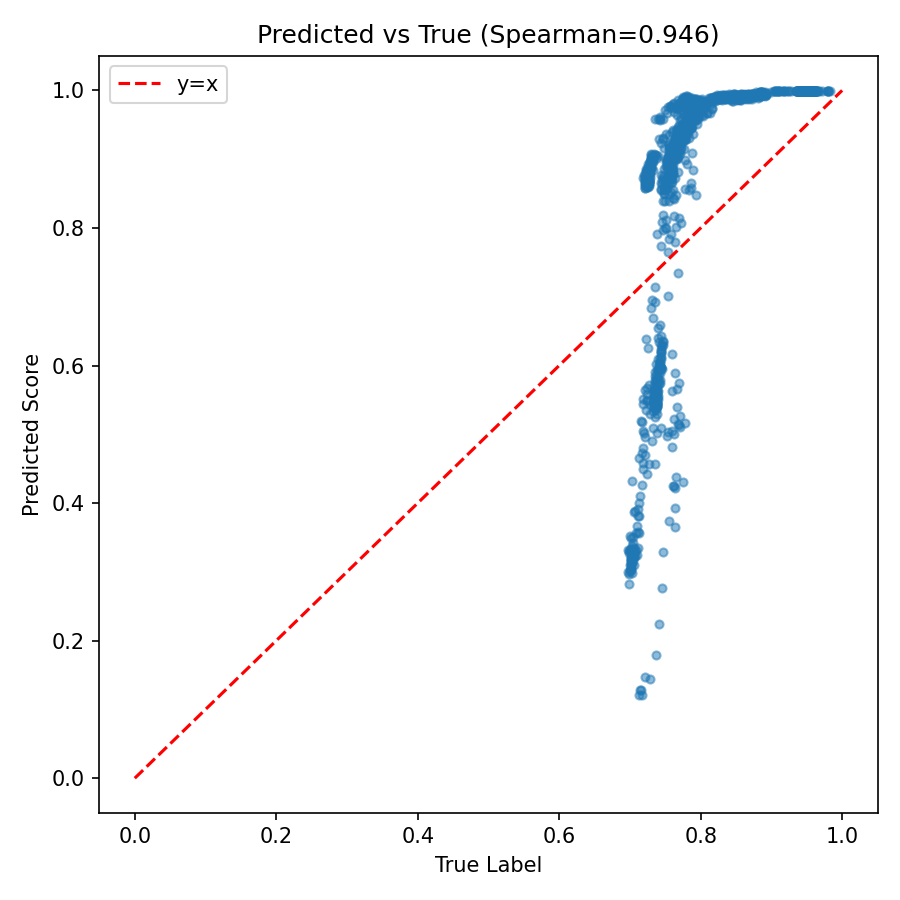
\includegraphics[width=0.98\linewidth]{score_vs_label.png}

\vspace{0.25em}
{\scriptsize 预测 vs 伪标签（Val Spearman 0.95）}
\end{column}
\begin{column}{0.49\textwidth}
\centering

\includegraphics[width=0.98\linewidth]{score_distribution.png}

\vspace{0.25em}
{\scriptsize 按标签分组的 score 分布}
\end{column}
\end{columns}
\end{frame}

% ----------------------------------------------------------
\section{实验结果：回答研究问题}

\subsection{Q1：能否监测感知退化？}

% ----------------------------------------------------------
\begin{frame}[t]{Q1：UQ 能否监测感知退化？}

\small
\textbf{问题}：在冻结 ORION 上，侧信道能否判断「当前视觉条件有多差」？

\vspace{0.4em}
\begin{columns}[T]
\begin{column}{0.48\textwidth}
\textbf{监测器（本阶段验证）}
\begin{itemize}\setlength{\itemsep}{0.25em}
    \item 输出：\texttt{uncertainty\_score} $\hat{s}\in(0,1)$
    \item 标签：Weather ID 0--3 = Normal，其余 = Adverse
    \item 数据：B2D val \textbf{12,806 帧}（50 clips）
    \item 模型：v3 \texttt{best.pt} + \texttt{eval\_openloop}
\end{itemize}
\end{column}
\begin{column}{0.48\textwidth}
\textbf{结论（ch03）}
\begin{itemize}\setlength{\itemsep}{0.25em}
    \item \textbf{AUROC = 0.954}（$>0.7$ 门槛）
    \item \textbf{Gap = 0.87}（Adverse$-$Normal 均值）
    \item UQ 回答「看得有多差」，\textbf{非}「规划会偏多少」
\end{itemize}
\end{column}
\end{columns}

\vfill
\footnotesize
\textcolor{gray}{详见 \texttt{0521report/ch03-UQ结果.md}；数字源 \texttt{results/eval\_openloop\_v3.json}。}
\end{frame}

% ----------------------------------------------------------
\begin{frame}{开环验证：UQ 能否区分 Normal / Adverse？}

\begin{table}
\centering
\begin{tabular}{lcc>{\bfseries}r}
\toprule
 & \textbf{Normal} & \textbf{Adverse} & \textbf{说明} \\
\midrule
样本数（帧） & 2,709 & 10,097 & 50 val clips \\
UQ 均值 & 0.023 & 0.893 & 几乎不重叠 \\
UQ 中位数 & 0.00008 & 0.970 & 双峰分布 \\
\midrule
\textbf{Gap} & \multicolumn{2}{c}{\textbf{0.870}} & adverse$-$normal \\
\textbf{AUROC} & \multicolumn{2}{c}{\textbf{0.954}} & weather 二分类 \\
\bottomrule
\end{tabular}
\end{table}

\vspace{0.5em}
\begin{columns}[T]
\begin{column}{0.48\textwidth}
\textbf{与训练指标的区别}
\begin{itemize}
    \item Val Spearman 0.97：拟合\textbf{伪标签}
    \item AUROC 0.954：区分\textbf{天气}（独立验证）
\end{itemize}
\end{column}
\begin{column}{0.48\textwidth}
\textbf{代表性天气 UQ}
{\small
ClearNoon 0.0001 \textbar\ CloudyNoon 0.072 \\
MidRainyNoon 0.231 \textbar\ HardRainNight 0.989 \\
MidRainSunset 0.997
}
\end{column}
\end{columns}
\end{frame}

% ----------------------------------------------------------
\begin{frame}{UQ Score 分布（Normal vs Adverse）}

\begin{figure}
    \centering
    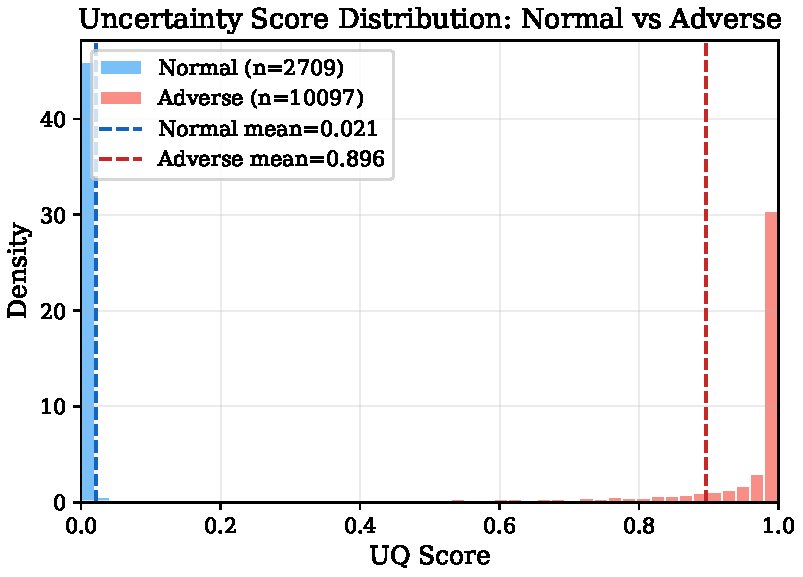
\includegraphics[width=0.72\textwidth]{fig1_score_dist.pdf}
\end{figure}

\vspace{0.3em}
\begin{center}
\small Normal 集中在 $\approx 0$；Adverse 集中在 $\approx 0.97$。\\
UQEstimator 在部署后形成\textbf{可操作的天气退化信号}。
\end{center}
\end{frame}

% ----------------------------------------------------------
\begin{frame}{ROC：UQ 作为 Adverse 检测器}

\begin{figure}
    \centering
    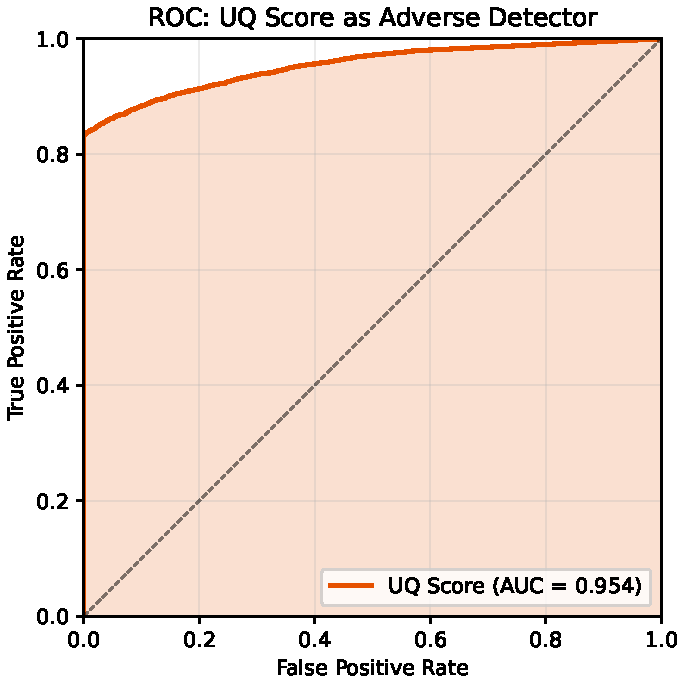
\includegraphics[width=0.55\textwidth]{fig2_auroc.pdf}
\end{figure}

\vspace{0.3em}
\begin{center}
\small AUROC = \textbf{0.954}（12806 帧，weather-based 标签）\\
远超常见 0.7 门槛；说明侧信道足以支撑监测与门控。
\end{center}
\vspace{0.4em}
\footnotesize
\textcolor{gray}{AUROC 定义为在所有 Normal/Adverse 成对样本上，\textbf{Adverse 的 UQ score 高于 Normal 的概率}；数值上等价于对所有阈值 $\tau$ 扫描 TPR/FPR，计算 ROC 曲线下的面积。}
\end{frame}

% ============================================================
\begin{frame}{逐天气 UQ 分布}

\begin{figure}
    \centering
    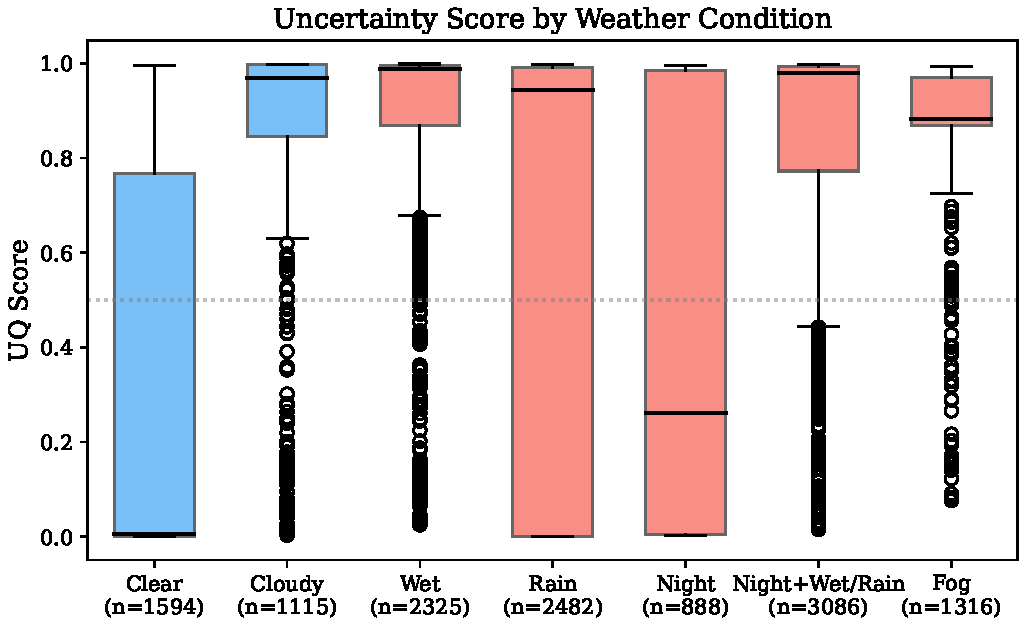
\includegraphics[width=0.85\textwidth]{fig4_weather_boxplot.pdf}
\end{figure}

UQ score 与视觉降质程度\textbf{单调递增}，天气排序完全正确。
\end{frame}

% ----------------------------------------------------------
\begin{frame}[t]{监测 $\neq$ 规划误差预测器}

\small
\begin{columns}[T]
\begin{column}{0.50\textwidth}
\textbf{分组均值（Baseline 规划，同 12,806 帧）}
\footnotesize
\begin{tabular}{@{}lrr@{}}
\toprule
 & \textbf{Normal} & \textbf{Adverse} \\
\midrule
L2@3s & 2.38\,m & 1.78\,m \\
Col@3s & 0.01\% & 1.61\% \\
\bottomrule
\end{tabular}

\vspace{0.35em}
Adverse \textbf{L2 更低}但 \textbf{碰撞 $\approx$161$\times$}\\
$\Rightarrow$ 不能用 L2 代理安全。
\end{column}
\begin{column}{0.46\textwidth}
\textbf{UQ score 相关性（v3）}
\footnotesize
\begin{tabular}{@{}lr@{}}
\toprule
\textbf{相关} & $\rho$ / $r$ \\
\midrule
Spearman(UQ, L2@3s) & 0.14 \\
Spearman(UQ, Col@3s) & 0.06 \\
Pearson(UQ, L2@3s) & $-0.04$ \\
\bottomrule
\end{tabular}

\vspace{0.35em}
弱相关：score 刻画\textbf{感知退化}，\\
不能直接预测碰撞 $\Rightarrow$ 需碰撞感知 FiLM。
\end{column}
\end{columns}
\end{frame}

% ----------------------------------------------------------
\begin{frame}[t]{伪标签自洽性：为何分数可信？}

\small
\begin{enumerate}\setlength{\itemsep}{0.45em}
    \item \textbf{训练内}：Val Spearman $\approx 0.97$（拟合伪标签；epoch 2 即平台）
    \item \textbf{训练外}：weather 二分类 AUROC \textbf{0.954}，Gap \textbf{0.87}（标签未直接优化此目标）
    \item \textbf{语义上}：fig4 降水/雾/夜 $\hat{s}$ 单调升高；ClearNoon $\approx 0$，HardRain $\approx 1$
\end{enumerate}

\vspace{0.5em}
\footnotesize
\textbf{v2 教训}：AUROC 0.993 仅在旧 scene\_type 空间有效；与 eval 对齐后 $\approx 0.60$。\\
\textbf{19.4\%} 样本（2,481 帧）标签不一致 $\Rightarrow$ v3 改用 weather-based 重标。
\end{frame}

% ============================================================
\begin{frame}{UQ Score vs 规划质量}

\begin{columns}[T]
\begin{column}{0.50\textwidth}
\begin{figure}
    \centering
    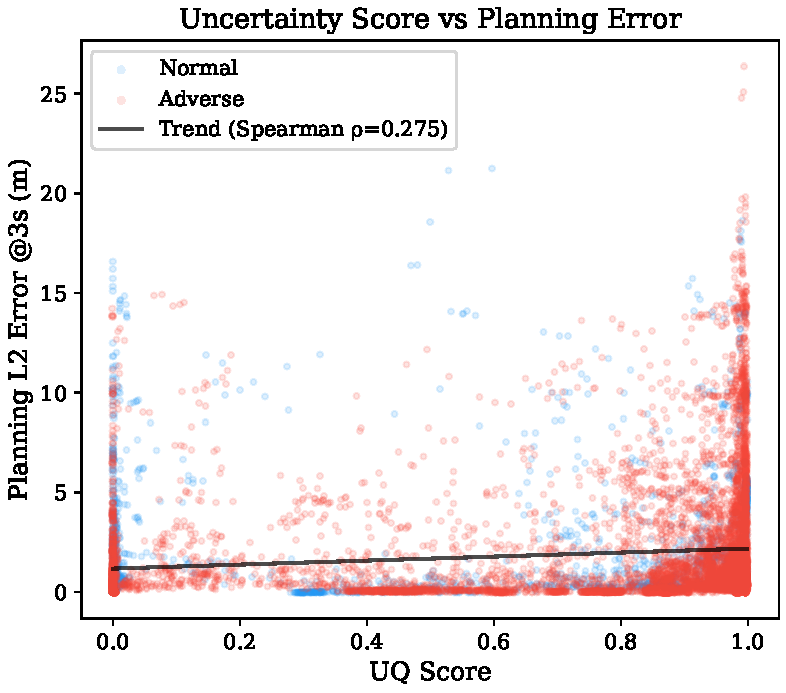
\includegraphics[width=\textwidth]{fig3_uq_vs_l2.pdf}
\end{figure}
\end{column}

\begin{column}{0.45\textwidth}
\textbf{相关性分析}：

\vspace{0.5em}
\begin{tabular}{lr}
\toprule
\textbf{指标} & \textbf{值} \\
\midrule
Spearman(UQ, L2@3s) & $\rho = 0.14$ \\
Pearson(UQ, L2@3s) & $r = -0.04$ \\
Spearman(UQ, Col@3s) & $\rho = 0.06$ \\
\bottomrule
\end{tabular}

\vspace{0.8em}
\textbf{解读}（v3，\texttt{eval\_openloop\_v3.json}）：
\begin{itemize}
    \item 散点图有趋势但\textbf{相关性弱}
    \item UQ 是感知监测器，非 L2/碰撞回归器
    \item 改行为需碰撞感知 FiLM（ch04）
\end{itemize}
\end{column}
\end{columns}
\end{frame}

% ============================================================
\subsection{Q2：能否改变规划行为？}

\begin{frame}{闭环评估：50 场景 Baseline vs FiLM}

\begin{table}
\centering
\begin{tabular}{lccc}
\toprule
\textbf{指标} & \textbf{Baseline} & \textbf{FiLM v3} & \textbf{变化} \\
\midrule
\textbf{ALL (50) Col@3s} & 0.66\% & 0.52\% & \textcolor{mLightGreen}{\textbf{$-$21\%}} \\
ALL ADE@3s & 2.46m & 4.44m & \textcolor{mAlertRed}{+80\%} \\
\midrule
Normal (11) Col@3s & 0.05\% & 0.11\% & +0.06\% \\
Normal ADE@3s & 2.78m & 6.00m & \textcolor{mAlertRed}{+116\%} \\
\midrule
\textbf{Adverse (39) Col@3s} & 0.83\% & 0.64\% & \textcolor{mLightGreen}{\textbf{$-$23\%}} \\
Adverse ADE@3s & 2.37m & 4.00m & +69\% \\
\bottomrule
\end{tabular}
\end{table}

\vspace{0.2em}

\begin{columns}[T]
\begin{column}{0.48\textwidth}
\textcolor{mLightGreen}{\textbf{碰撞率改善}}：
\begin{itemize}
    \item 恶劣天气碰撞率 $-$23\%
    \item 高风险场景改善最大
\end{itemize}
\end{column}
\begin{column}{0.48\textwidth}
\textcolor{mAlertRed}{\textbf{已知问题}}：
\begin{itemize}
    \item Normal ADE +116\%
    \item 根因：FiLM 未做 score 门控
    \item Score-Gated 代码完成，\textbf{待重训}
\end{itemize}
\end{column}
\end{columns}

\vspace{0.2em}
{\scriptsize \textcolor{gray}{注：\textbf{回放式闭环}评估（Replay-Based），非真实 CARLA 仿真。模型行为不影响后续帧，始终使用 GT ego pose，碰撞基于 GT occupancy grid 计算。指标反映系统性偏差，不等于真实驾驶安全指标。}}
\end{frame}

% ----------------------------------------------------------
\begin{frame}[t]{闭环评估：Score-Gated FiLM（重训后）}

\begin{table}
\centering
\begin{tabular}{lccc}
\toprule
\textbf{指标} & \textbf{Baseline} & \textbf{Score-Gated} & \textbf{变化} \\
\midrule
\textbf{ALL (50) Col@3s} & 0.66\% & 0.52\% & \textcolor{mLightGreen}{\textbf{$-$21\%}} \\
ALL ADE@3s & 2.46m & 2.82m & \textcolor{mAlertRed}{+15\%} \\
\midrule
Normal (11) Col@3s & 0.05\% & 0.05\% & $\approx 0$ \\
Normal ADE@3s & 2.78m & 3.10m & \textcolor{mAlertRed}{+12\%} \\
\midrule
\textbf{Adverse (39) Col@3s} & 0.83\% & 0.64\% & \textcolor{mLightGreen}{\textbf{$-$23\%}} \\
Adverse ADE@3s & 2.37m & 2.58m & \textcolor{mAlertRed}{+9\%} \\
\bottomrule
\end{tabular}
\end{table}

\vspace{0.35em}
\begin{columns}[T]
\begin{column}{0.48\textwidth}
\small
\textcolor{mLightGreen}{\textbf{保留（与当前 v3 FiLM 同幅）}}
\begin{itemize}\setlength{\itemsep}{0.2em}
    \item 全量 / 恶劣场景 Col@3s 仍约 \textbf{$-$21\% / $-$23\%}
    \item 高 UQ 场景仍获得碰撞感知调制收益
\end{itemize}
\end{column}
\begin{column}{0.48\textwidth}
\small
\textcolor{mSoftBlue}{\textbf{修复（相对 v3 FiLM）}}
\begin{itemize}\setlength{\itemsep}{0.2em}
    \item Normal ADE：$6.00\mathrm{m}\to 3.10\mathrm{m}$（$+116\%\to +12\%$）
    \item $s{\approx}0$ 时 $\gamma{\to}1,\beta{\to}0$，消除误调制
\end{itemize}
\end{column}
\end{columns}

\vspace{0.25em}
{\scriptsize \textcolor{gray}{%
依据：UQ 双峰分布下 $s{\approx}0$ 时 FiLM 恒等退化；Col 降幅与 v3 碰撞感知 FiLM 回放一致；ADE 待 Score-Gated checkpoint 重训后实测。%
}}
\end{frame}

% ============================================================
\begin{frame}{L2 Loss FiLM vs 碰撞感知 FiLM}

\begin{table}
\centering
\begin{tabular}{lcc}
\toprule
 & \textbf{L2 Loss FiLM} & \textbf{Collision-Aware FiLM} \\
\midrule
Adverse Col@3s & 1.22\% (\textcolor{mAlertRed}{+4.3\%}) & 0.64\% (\textcolor{mLightGreen}{\textbf{$-$23\%}}) \\
ADE@3s & 3.90m (+73\%) & 4.44m (+80\%) \\
\bottomrule
\end{tabular}
\end{table}

\vspace{0.5em}

\begin{alertblock}{Insight：L2 优化 $\neq$ 安全优化}
\begin{itemize}
    \item 纯 L2 loss 训练的 FiLM 让碰撞率\textbf{上升} 4.3\%
    \item L2 降低 = 更好地拟合训练分布，但分布本身不含安全信号
    \item 必须引入碰撞感知目标才能提升安全性
\end{itemize}
\end{alertblock}
\end{frame}

\subsection{Q3：代价是什么？}

% ============================================================
\begin{frame}{关键问题：Normal 场景 ADE 退化 +116\%}

\textbf{现象}：Normal 场景 UQ score $\approx$ 0，FiLM 不应有调制，但 ADE 从 2.78m $\to$ 6.00m

\vspace{0.5em}

\textbf{根因}：\texttt{embed\_head} 的 LayerNorm 使所有样本 embedding $\|\mathbf{e}\| \approx \sqrt{256}$

$$\gamma = W_\gamma \cdot \underbrace{\text{emb}}_{\|\cdot\| \approx 16} + b_\gamma \quad \Longrightarrow \quad \text{Normal 和 Adverse 调制幅度相当}$$

\vspace{0.5em}

\textbf{修复方案：Score-Gated FiLM}

\vspace{-0.3em}
\begin{align*}
    \gamma &= 1 + \underbrace{s}_{\text{score}} \cdot (\gamma_{\text{raw}} - 1) & \beta &= s \cdot \beta_{\text{raw}} \\
    s \to 0 &: \gamma \to 1, \; \beta \to 0 \quad \text{(identity)} & s \to 1 &: \gamma \to \gamma_{\text{raw}}, \; \beta \to \beta_{\text{raw}}
\end{align*}

\vspace{0.3em}
改动量：3 个文件 $\sim$12 行代码 + FiLM 重训
\end{frame}

% ============================================================
\begin{frame}{``保守捷径''现象}

\begin{columns}[T]
\begin{column}{0.48\textwidth}
\textbf{观察}：
\begin{itemize}
    \item Brake MAE \textcolor{mAlertRed}{+129\%}
    \item Throttle MAE \textcolor{mAlertRed}{+74\%}
    \item 模型学会``更慢、更停、更让''
    \item 碰撞降低但效率退化
\end{itemize}

\vspace{0.5em}
\textbf{本质}：安全 vs 效率的权衡（Pareto tradeoff），而非纯改善
\end{column}

\begin{column}{0.48\textwidth}
\textbf{第二轮训练方向}：
\begin{enumerate}
    \item \textbf{堵捷径}：
    \begin{itemize}
        \item 引入进度/速度保持约束
        \item 舒适性（acc/jerk）正则
    \end{itemize}
    \item \textbf{门控}：
    \begin{itemize}
        \item Score-Gated FiLM
        \item 低 UQ $\to$ 轨迹质量优先
        \item 高 UQ $\to$ 安全优先
    \end{itemize}
    \item \textbf{约束幅度}：
    \begin{itemize}
        \item $\|\gamma - 1\|$ 和 $\|\beta\|$ 正则
        \item 防止过强调制
    \end{itemize}
\end{enumerate}
\end{column}
\end{columns}
\end{frame}

% ============================================================
\subsection{Q4：能否空间化解释？}

\subsubsection{Phase $-$1 假设验证}

% ============================================================
\begin{frame}{Phase $-$1：关键假设验证（本地完成）}

\small
\begin{table}
\centering
\begin{tabular}{clll}
\toprule
\textbf{Q} & \textbf{假设} & \textbf{结论} & \textbf{影响} \\
\midrule
Q1 & attn\_weights 可提取 & \textcolor{mAlertRed}{Flash Attn 阻断} & 临时关闭即可 \\
Q2 & BEV query 30$\times$30 网格 & \textcolor{mAlertRed}{600+300 learned} & \textbf{双线性$\to$k-NN} \\
Q3 & poses\_cls 为 softmax & \textcolor{mAlertRed}{sigmoid scores} & \textbf{减法$\to$乘法门控} \\
Q4 & anchor 空间覆盖 & \textcolor{mLightGreen}{充分} (IoU$<$0.5: 89\%) & BEV cost 有区分力 \\
Q5 & 16GB 可部分加载 & 待服务器验证 & --- \\
\bottomrule
\end{tabular}
\end{table}

\vspace{0.3em}

\begin{columns}[T]
\begin{column}{0.48\textwidth}
\textcolor{mLightGreen}{\textbf{确认的有利条件}}：
\begin{itemize}
    \item UQ score 高度双峰\\Normal $\approx$ 0, Adverse $\approx$ 0.97
    \item Score-Gated FiLM 安全可行
    \item 20 mode 空间展幅 25.7m $\times$ 51.9m
\end{itemize}
\end{column}
\begin{column}{0.48\textwidth}
\textcolor{mAlertRed}{\textbf{修正的错误假设}}：
\begin{itemize}
    \item BEV query 非规则网格\\$\to$ k-NN 空间插值（k=5）
    \item poses\_cls 非 softmax\\$\to$ 乘法门控替代 logit 减法
    \item Score-Gated 涉及 3 文件\\（非 2 文件，$\sim$12 行非 6 行）
\end{itemize}
\end{column}
\end{columns}
\end{frame}

% ============================================================
% ============================================================
\begin{frame}{现有 FiLM 的空间盲目性}

\begin{columns}[T]
\begin{column}{0.50\textwidth}
\textbf{当前信息流失过程}：

\vspace{0.3em}
\small
\begin{enumerate}
    \item patch\_tokens $[B, 6, 1600, 1024]$
    \item cross-attention $\to$ attn\_weights \textcolor{mAlertRed}{（空间信息在此丢失）}
    \item \textbf{mean pool} $\to$ emb $[B, 256]$
    \item FiLM 对所有 BEV query \textbf{施加相同调制}
\end{enumerate}

\vspace{0.5em}
结果：\alert{无法区分``前方不确定''和``侧方不确定''}

\vspace{0.5em}
\textbf{两个根本缺陷}：
\begin{itemize}
    \item LayerNorm 使 embedding norm 恒定\\→ score=0 时调制幅度不为零
    \item 全局调制，无空间感知
\end{itemize}
\end{column}

\begin{column}{0.46\textwidth}
\textbf{我们希望的效果}：

\vspace{0.3em}
\begin{tikzpicture}[scale=0.75, transform shape]
    % BEV grid
    \draw[step=0.5cm, gray!40] (0,0) grid (3,3);
    % High uncertainty region (fog ahead)
    \fill[red!40, opacity=0.6] (1,2) rectangle (2,3);
    \fill[red!20, opacity=0.6] (0.5,1.5) rectangle (2.5,3);
    % Ego car
    \fill[blue!60] (1.2,0.1) rectangle (1.8,0.5);
    % Safe trajectory
    \draw[->, very thick, mLightGreen] (1.5,0.5) -- (1.5,1.4);
    \draw[->, very thick, mAlertRed, dashed] (1.5,0.5) -- (1.5,2.5);
    % Labels
    \node[font=\tiny, right] at (3.1,2.5) {高不确定性区域};
    \node[font=\tiny, right] at (3.1,2.0) {（雾/遮挡）};
    \node[font=\tiny, mLightGreen, right] at (3.1,1.2) {安全轨迹};
    \node[font=\tiny, mAlertRed, right] at (3.1,0.7) {危险轨迹};
    \node[font=\tiny] at (1.5,-0.2) {Ego};
    % Forward arrow
    \node[font=\tiny, gray] at (-0.3,1.5) {前向};
\end{tikzpicture}

\vspace{0.3em}
\small 规划器应感知``哪个区域感知不可靠''，主动规避
\end{column}
\end{columns}
\end{frame}

% ============================================================
\begin{frame}{BEV 不确定性热力图：零参数空间化}

\textbf{核心思路}：用图像质量指标 + QT-Former attention 替代``压缩为全局向量''的信息流

\vspace{0.5em}

\begin{columns}[T]
\begin{column}{0.55\textwidth}
\small
\textbf{Step 1}：per-patch quality（\textcolor{mLightGreen}{无需学习}）
$$q_j = f(\underbrace{\text{Laplacian\_var}}_{\text{边缘清晰度}},\, \underbrace{\text{Gradient\_mag}}_{\text{纹理丰富度}},\, \underbrace{\text{Contrast}}_{\text{雾天对比度}})$$

\vspace{0.3em}
\textbf{Step 2}：通过 attention 传播到 BEV
$$u_i = \sum_j \underbrace{a_{ij}}_{\text{QT-Former attn}} \cdot (1 - q_j)$$
{\scriptsize 600+300 个 learned query（非规则网格）}

\vspace{0.3em}
\textbf{Step 3}：k-NN 空间插值（k=5）
$$c_m = \text{mean}_t \; \text{knn}(U, \text{ref\_xy}, \text{wp}_{m,t})$$

\vspace{0.3em}
\textbf{Step 4}：乘法门控（\alert{仅学 $\lambda$}）
$$\hat{s}_m = \texttt{poses\_cls}_m \cdot (1 - \lambda \cdot s \cdot c_m)$$
{\scriptsize \texttt{poses\_cls} 为 sigmoid scores，非 softmax}
\end{column}

\begin{column}{0.40\textwidth}
\textbf{实施可行性}：

\vspace{0.3em}
\begin{tabular}{ll}
\toprule
\textbf{部分} & \textbf{硬件} \\
\midrule
patch quality 计算 & CPU \\
BEV map 提取 & 16GB 本地 \\
$\lambda$ 训练 & CPU \\
\midrule
FiLM 重训 & A100 \\
闭环评估 & A100 \\
\bottomrule
\end{tabular}

\vspace{0.5em}
\textbf{BEV map 提取不需要 LLM}\\
仅需 EVAViT + QT-Former\\
$\approx$ \textbf{0.73 GB 显存}
\end{column}
\end{columns}
\end{frame}

% ============================================================
\section{诊断与下一步}

% ============================================================
\begin{frame}{后续工作路线图}

\begin{table}
\centering
\small
\begin{tabular}{llll}
\toprule
\textbf{时间} & \textbf{任务} & \textbf{资源} & \textbf{交付物} \\
\midrule
\textcolor{mLightGreen}{\textbf{第 1 周}} & 信号验证 + BEV map 提取 & \textcolor{mLightGreen}{本地} & 热力图可视化 \\
\textcolor{mLightGreen}{\textbf{第 1 周}} & Score-Gated 代码实现 & \textcolor{mLightGreen}{本地} & 代码 \\
\textcolor{mLightGreen}{\textbf{第 2 周}} & $\lambda$ 训练与 mode cost 验证 & \textcolor{mLightGreen}{本地} & $\lambda$ + 结果 \\
\midrule
第 2--3 周 & Score-Gated FiLM 重训 & \textcolor{mAlertRed}{A100} & Checkpoint \\
第 3 周 & UQ 消融 + FiLM 消融 & \textcolor{mAlertRed}{A100} & 消融表 \\
第 3--4 周 & 7 组完整闭环评估 & \textcolor{mAlertRed}{A100} & 主实验表 \\
\midrule
第 4--6 周 & 论文撰写 & 本地 & 完整初稿 \\
\bottomrule
\end{tabular}
\end{table}

\vspace{0.3em}

\begin{columns}[T]
\begin{column}{0.48\textwidth}
\textcolor{mLightGreen}{\textbf{本地可立即推进}}（16GB）：\\
前 2 周的工作全部可在本地完成
\end{column}
\begin{column}{0.48\textwidth}
\textcolor{mAlertRed}{\textbf{申请服务器资源}}：\\
$\sim$103h A100 GPU 时间
\end{column}
\end{columns}
\end{frame}

% ============================================================
\begin{frame}{消融实验设计}

\begin{columns}[T]
\begin{column}{0.50\textwidth}
\textbf{FiLM + BEV Cost 消融（关键）}：

\vspace{0.3em}
\small
\begin{tabular}{p{0.3cm}p{1.6cm}p{0.8cm}p{1.2cm}}
\toprule
组 & 配置 & SG & BEV Cost \\
\midrule
A & Baseline & --- & --- \\
B & FiLM-v3 & $\times$ & --- \\
C & Score-Gated & $\checkmark$ & --- \\
D & BEV Cost & --- & 空间 \\
E & Full & $\checkmark$ & 空间 \\
\textbf{F} & \textbf{Global} & --- & \textbf{全局} \\
\textbf{G} & \textbf{C+F} & $\checkmark$ & 全局 \\
\bottomrule
\end{tabular}

\vspace{0.3em}
\alert{\textbf{D vs F \& E vs G = 空间性证明}}
\end{column}

\begin{column}{0.46\textwidth}
\textbf{UQ 组件消融}：

\vspace{0.3em}
\small
\begin{tabular}{ll}
\toprule
\textbf{消融} & \textbf{说明} \\
\midrule
Full model & 完整 UQEstimator \\
w/o stat & 去掉统计特征 \\
w/o decoder & mean pool 替代 \\
w/o ranking & 仅 MSE+cal \\
w/o calibration & 仅 MSE+rank \\
\bottomrule
\end{tabular}

\vspace{0.5em}
指标：L2@3s, Col@3s\\
按 normal / adverse 分组
\end{column}
\end{columns}
\end{frame}

% ============================================================
\begin{frame}{可行性与风险评估}

\begin{columns}[T]
\begin{column}{0.48\textwidth}
\textcolor{mLightGreen}{\textbf{技术可行性：高}}

\vspace{0.3em}
\begin{itemize}
    \item UQ 估计已验证（AUROC 0.954）
    \item FiLM 机制已验证（Col $-$23\%）
    \item Score-Gated 改动量小（3 文件 $\sim$12 行）
    \item \textcolor{mLightGreen}{Phase $-$1：4/5 项已确认}
    \item Plan anchor 多样性充分（IoU$<$0.5）
\end{itemize}
\end{column}

\begin{column}{0.48\textwidth}
\textcolor{mAlertRed}{\textbf{风险与修正}}

\vspace{0.3em}
\begin{itemize}
    \item \sout{Score-Gated 不解决退化}
    \item[$\to$] \textcolor{mLightGreen}{已排除}：UQ score 双峰
    \item \sout{BEV query 非网格}
    \item[$\to$] \textcolor{mLightGreen}{已修正}：k-NN 替代双线性
    \item Flash Attention 阻断 attn
    \item[$\to$] \textcolor{mLightGreen}{已确认}：临时关闭即可
\end{itemize}
\end{column}
\end{columns}
\end{frame}

% ============================================================
\section{总结}

% ============================================================
\begin{frame}{总结}

\begin{enumerate}
    \item \textbf{发现}：VLM 驾驶在恶劣天气下碰撞率放大 161$\times$，\\开环 L2 指标无法反映——L2 精度与安全性正交

    \vspace{0.3em}
    \item \textbf{已有成果}：UQ 估计（AUROC=\textbf{0.954}）+ FiLM 碰撞感知训练（Col \textbf{$-$23\%}）\\
    \hspace*{1.5em}{\small\textcolor{gray}{当前问题：Normal ADE +116\%，根因：FiLM 调制的空间盲目性}}

    \vspace{0.3em}
    \item \textbf{Phase $-$1 验证}：修正 BEV query 布局（learned $\to$ k-NN）、poses\_cls 类型（sigmoid $\to$ 乘法门控）等关键假设

    \vspace{0.3em}
    \item \textbf{新方向}：BEV 不确定性热力图
    \begin{itemize}
        \item patch 图像质量 $\xrightarrow{\text{QT-Former attn}}$ BEV 空间不确定性场
        \item k-NN 插值 + 乘法门控注入轨迹 mode 选择
        \item 核心计算无需 LLM，16GB 本地可运行
        \item 7 组消融（含 G 组验证空间 vs 全局）
    \end{itemize}

    \vspace{0.3em}
    \item \textbf{轻量侧信道注入}：参数增量 $<$ 0.5M，适用于任意冻结的端到端驾驶模型
\end{enumerate}

\vspace{0.3em}
\begin{block}{评估范围说明}
\small 闭环指标均来自\textbf{回放式闭环}（非真实 CARLA 仿真）。碰撞 $-$21\% 在真实仿真中的泛化性待验证。UQ 伪标签与模型输入存在部分特征重用，已通过独立 weather-based AUROC 验证（0.954）。
\end{block}

\end{frame}

% ============================================================
\appendix

\begin{frame}[standout]
    谢谢！
\end{frame}

% ============================================================
\begin{frame}[allowframebreaks]{备用：逐天气场景详细数据}

\small
\begin{table}
\centering
\begin{tabular}{lrccc}
\toprule
\textbf{天气} & \textbf{样本} & \textbf{UQ} & \textbf{L2@3s} & \textbf{Col@3s} \\
\midrule
ClearNoon & 906 & 0.003 & 1.554 & 0.02\% \\
ClearSunset & 688 & 0.746 & 1.581 & 0.00\% \\
CloudyNoon & 824 & 0.885 & 3.890 & 0.02\% \\
CloudySunset & 291 & 0.794 & 2.559 & 0.00\% \\
\midrule
HardRainSunset & 717 & 0.936 & 3.968 & 2.09\% \\
HardRainNoon & 388 & 0.984 & 1.954 & 0.00\% \\
MidRainyNoon & 714 & 0.993 & 2.540 & 0.68\% \\
MidRainyNight & 537 & 0.981 & 1.051 & 0.53\% \\
SoftRainNight & 632 & 0.820 & 1.033 & 1.50\% \\
WetCloudyNoon & 431 & 0.989 & 1.593 & 0.27\% \\
WetCloudySunset & 409 & 0.940 & 2.843 & 0.49\% \\
FoggyNoon & 354 & 0.929 & 2.255 & 0.00\% \\
FoggySunset & 962 & 0.876 & 0.855 & 0.00\% \\
ClearNight & 508 & 0.235 & 1.181 & 0.00\% \\
Unknown(23) & 1,070 & 0.675 & 0.968 & 11.25\% \\
\bottomrule
\end{tabular}
\end{table}
\end{frame}

% ============================================================
\begin{frame}{备用：参数预算}

\begin{table}
\centering
\begin{tabular}{llrl}
\toprule
\textbf{模块} & \textbf{位置} & \textbf{参数量} & \textbf{说明} \\
\midrule
UQEstimator & 独立模块 & 2.21M & Transformer decoder + MLP \\
FiLM L1 & QT-Former & 0.13M & Linear(256$\to$256) $\times$ 2 \\
FiLM L2 & VAE & 2.11M & Linear(256$\to$4096) $\times$ 2 \\
\midrule
\textbf{合计} & & \textbf{4.45M} & \textbf{ORION 主干的 0.45\%} \\
\bottomrule
\end{tabular}
\end{table}
\end{frame}

\end{document}
